% Build this with LuaLaTeX or see below.

% Mandatory if you want to build in LuaLaTeX with the `standalone`class
% just remove it to build with another engine.
\RequirePackage{luatex85}
\documentclass[crop,tikz]{standalone}  % You can obviously change this to any class you want
% The following four lines are required, since we use those libraries
\usepackage{tikz}
    \usetikzlibrary{positioning}
    \usetikzlibrary{calc}
    \usetikzlibrary{shapes.multipart}

\begin{document}
% You can put your own tikzpicture instead of this one, which is the one `ginger` generates from `example.conll`
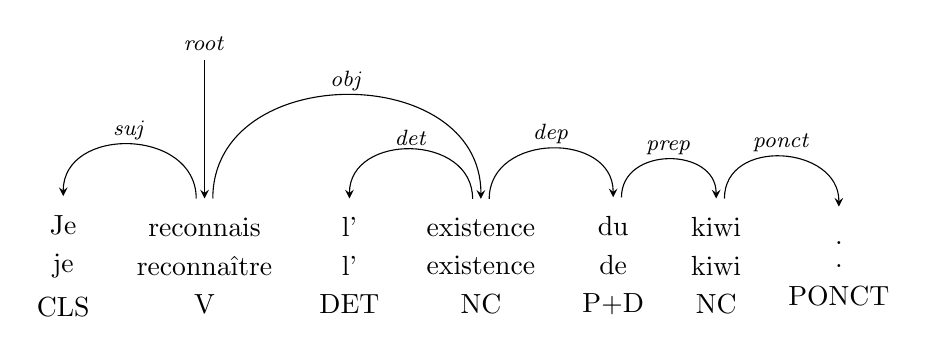
\begin{tikzpicture}[>=stealth, token/.style={text height=1em, rectangle split, rectangle split parts=3}]
\path[anchor=base]
    node[token] (t1) {Je\nodepart{two}je\nodepart{three}CLS}
    node[token, right=1em of t1] (t2) {reconnais\nodepart{two}reconnaître\nodepart{three}V}
    node[token, right=1em of t2] (t3) {l'\nodepart{two}l'\nodepart{three}DET}
    node[token, right=1em of t3] (t4) {existence\nodepart{two}existence\nodepart{three}NC}
    node[token, right=1em of t4] (t5) {du\nodepart{two}de\nodepart{three}P+D}
    node[token, right=1em of t5] (t6) {kiwi\nodepart{two}kiwi\nodepart{three}NC}
    node[token, right=1em of t6] (t7) {.\nodepart{two}.\nodepart{three}PONCT};
    \begin{scope}[local bounding box=arcs]
        \draw[->] let \p1 = ($(t2)-(t1)$) in ($(t2.north)+(-.3em, 0)$) ..  controls ($(t2.north)+(-.3em, {abs(\x1)*0.5})$) and ($(t1.north)+(0, {abs(\x1)*0.5})$) ..
    (t1.north) node[midway, above=-.2em] {\footnotesize\emph{suj}};
        \draw[->] let \p1 = ($(t4)-(t3)$) in ($(t4.north)+(-.3em, 0)$) ..  controls ($(t4.north)+(-.3em, {abs(\x1)*0.5})$) and ($(t3.north)+(0, {abs(\x1)*0.5})$) ..
(t3.north) node[midway, above=-.2em] {\footnotesize\emph{det}};
        \draw[->] let \p1 = ($(t2)-(t4)$) in ($(t2.north)+(.3em, 0)$) ..  controls ($(t2.north)+(.3em, {abs(\x1)*0.5})$) and ($(t4.north)+(0, {abs(\x1)*0.5})$) .. (t4.north) node[midway, above=-.2em] {\footnotesize\emph{obj}};
        \draw[->] let \p1 = ($(t4)-(t5)$) in ($(t4.north)+(.3em, 0)$) ..  controls ($(t4.north)+(.3em, {abs(\x1)*0.5})$) and ($(t5.north)+(0, {abs(\x1)*0.5})$) .. (t5.north) node[midway, above=-.2em] {\footnotesize\emph{dep}};
        \draw[->] let \p1 = ($(t5)-(t6)$) in ($(t5.north)+(.3em, 0)$) ..  controls ($(t5.north)+(.3em, {abs(\x1)*0.5})$) and ($(t6.north)+(0, {abs(\x1)*0.5})$) .. (t6.north) node[midway, above=-.2em] {\footnotesize\emph{prep}};
        \draw[->] let \p1 = ($(t6)-(t7)$) in ($(t6.north)+(.3em, 0)$) ..  controls ($(t6.north)+(.3em, {abs(\x1)*0.5})$) and ($(t7.north)+(0, {abs(\x1)*0.5})$) .. (t7.north) node[midway, above=-.2em] {\footnotesize\emph{ponct}};
    \end{scope}

    \draw[->] ($(arcs.north west)!(t2.north)!(arcs.north east)$) node[above] {\footnotesize\emph{root}} -- (t2.north);
\end{tikzpicture}
\end{document}
